\section{Reproducibility in Scientific Workflows}
\label{sec:reproducibility}

In this section, we introduce the tools used for the instantiation and evaluation 
of the aforementioned semantic models. We first describe the Pegasus Workflow 
Management System (WMS)~\cite{Pegasus, Deelman-FGCS-2014}, which is used as our 
workflow engine, and then a set of reproducibility tools for semantic annotations and 
experiment management.


\subsection{Scientific Workflow Execution}

The Pegasus WMS can manage workflows comprised of millions of tasks, recording data 
about their execution and intermediate results. In Pegasus, workflows are described as 
abstract workflows, that is, they do not contain resource information, or the physical locations of 
data and executables. Workflows are described as directed acyclic graphs (DAGs), where 
nodes represent individual computational tasks and the edges represent data and control 
dependencies between tasks. The abstract workflow description is represented as a DAX 
(DAG in XML), capturing all the tasks that perform computations, the execution order of these 
tasks, and for each task the required inputs, expected outputs, and the arguments with which 
the task should be invoked. 

During a workflow execution, Pegasus translates an abstract workflow into an 
executable workflow, determining the executables, data, and computational resources 
required for the execution. Pegasus maps executables to their installation paths or to a 
repository of stageable binaries defined in a Transformation Catalog (TC). A workflow 
execution includes data management, monitoring, and failure handling. Individual workflow 
tasks are managed by a task scheduler (HTCondor~\cite{condor}), which supervises their 
execution on local and remote resources.


\subsection{Reproducibility Artifacts}

To conduct the experimentation on scientific workflows reproducibility, we 
use the WICUS framework~\cite{wicus}, which comprises the semantic models described 
in Section~\ref{sec:semantic} and a set of tools for annotating and consuming data; and 
the PRECIP~\cite{Azarnoosh-CRC-2013} experiment management tool to manage the 
experiment. In addition, we use Vagrant~\cite{palat2012introducing}, a tool for deploying virtual
deployment environments,  to achieve local reproducibility of the experiments. 
Below, we describe each of these tools in detail.


\subsubsection{WICUS}
\label{subsec:wicus}

The Workflow Infrastructure Conservation Using Semantics ontology 
(WICUS) is an OWL2 (Web Ontology Language) ontology network that 
implements the semantic models introduced in Section~\ref{sec:semantic}. This ontology 
network is available online~\cite{wicus-online} and its goal is to define the relevant and 
required properties for describing scientific computational infrastructures. 
The detailed description of the ontologies, including \rev{their } main terms and relation
in the context of a workflow execution are provided in~\cite{wicus}.
Currently, two versions of the ontology network have been released. The latest one, released in
August 2014,  includes a set of new properties for better describing software and hardware requirements, 
and \rev{also for } including the output information of a configuration process (e.g., the resultant IP and port \rev{on }
which a recently deployed service will be listening).


Besides the ontology network, a set of components have been developed around it, 
for facilitating the annotation of the resources involved \rev{in } the execution of a scientific workflow. 
These tools are not fully automated yet, but represent a first step \rev{in } helping users define the requirements of their 
experiments. Figure~\ref{fig:wicusflow} shows the main modules, their flow and intermediate 
results involved in the process for achieving reproducibility. \rev{It also } describes the process of 
data generation and consumption. Below, we provide an overview of each of these modules:

\begin{figure}[!htb]
	\centering
	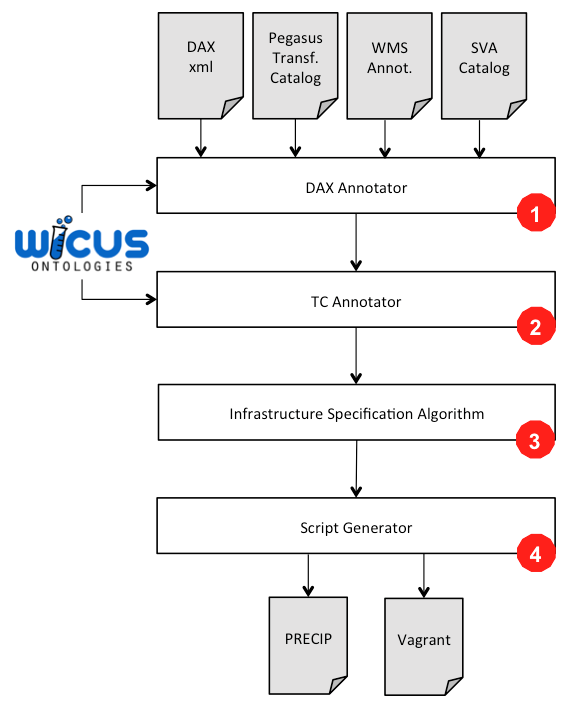
\includegraphics[width=.8\linewidth]{figures/wicusflow}
	\caption{WICUS annotation modules and flow. White boxes represent tools for semantic annotation or algorithms, and grey boxes represent files used or generated by the framework.}
	\label{fig:wicusflow}
\end{figure}

\begin{enumerate}
	\item \textbf{DAX Annotator.} This tool parses a DAX (Pegasus' workflow description) 
		and generates a set of annotations using the terms of the WICUS vocabulary, 
		representing workflow transformations and the workflow infrastructure requirements.

	\item \textbf{Workflow Annotations.} This RDF file contains the description of the workflow 
		and its infrastructure requirements.

	\item \textbf{WMS Annotations.} This RDF file contains the information of the WMS component 
		and its dependencies. This information is added to the \emph{Software Components 
		Catalog}.

	\item \textbf{Transformation Catalog Annotator.} This tool parses the Pegasus Transformation 
		Catalog (which describes the binaries involved on the workflow execution and their locations) 
		and the WMS annotations file, to generate two set of annotations: the \emph{Software 
		Components Catalog} and the \emph{Workflow \& Configuration Annotation} files.

	\item \textbf{Software Components Catalog.} This RDF file contains the set of annotations about 
		the binaries, dependencies, deployment plans and scripts, and configuration information of 
		the software involved in the experiment.

	\item \textbf{Workflow \& Configuration Annotation File.} This RDF file contains the same information 
		as in 2, but enriched with the configuration information for each workflow execution step, as 
		specified in the transformation catalog.

	\item \textbf{Scientific Virtual Appliances Catalog.} This RDF file contains available VM appliances. 
		Information about the related infrastructure providers and the VM images that compose an 
		appliance are included in this dataset.

	\item \textbf{Infrastructure Specification Algorithm.} This process reads files 5, 6, and 7, and 
		generates a configuration file, which describes VMs and software 
		components to be created and deployed.

	\item \textbf{Abstract Deployment Plan.} This plan contains information about the set of components 
		and their associated deployment steps for configuring the execution infrastructure. This plan 
		will be later enacted using a concrete language. This decoupled approach allows the integrations of
		new enactment  systems easily.
		
	\item \textbf{Script Generator.} This module concretizes the abstract deployment plan using the selected
		language (either PRECIP or Vagrant in this case) to generate an executable script. New script syntaxes 
		may be added in the future.

	\item \textbf{Executable Script.} This script creates a PRECIP/Vagrant experiment, which runs a VM, 
		copies the required binaries, and executes deployment scripts to set the environment for the 
		workflow execution. It also contains the original experiment commands in order to 
		re-execute it.

\end{enumerate}

In the experimentation process (Section~\ref{sec:experiment}), we will present a detailed description 
and the applicability of each module for the \rev{target } scientific workflows.



% PRECIP
\subsubsection{PRECIP}
The Pegasus Repeatable Experiments for the Cloud in Python (PRECIP)~\cite{Azarnoosh-CRC-2013} 
is a flexible experiment management control API for running experiments on all types of Clouds, 
including academic Clouds such as FutureGrid~\cite{futuregrid} and the NSFCloud~\cite{chameleon,cloudlab}
(through OpenStack), and commercial Clouds such as Amazon EC2~\cite{aws} and Google 
Compute Engine~\cite{gce}. In PRECIP, interactions with the provisioned instances are done by 
tagging. When an instance is provisioned, the scientist can add arbitrary tags to that instance in 
order to identify and group the instances in the experiment. API methods such as running remote 
commands, or copying files, all use tags to specify which instances to target. PRECIP does not 
force the scientist to use a special VM image, and no PRECIP components need to be pre-installed 
in the image. Scientists can use any basic Linux image and PRECIP will bootstrap instances using 
SCP and SSH commands. PRECIP provides functionality to run user-defined scripts on the instances 
to install/configure software and run experiments, and also manages SSH keys and security groups 
automatically.

In this work, we use PRECIP to define a script able to reproduce the execution environment of the 
former experiment, and run it on a Cloud platform.


% Vagrant
\subsubsection{Vagrant}

Vagrant~\cite{palat2012introducing} is an open-source and multi-platform solution for deploying 
development environments locally using virtualization. It relies on virtualization solutions such as 
Oracle VirtualBox~\cite{Watson2008} (also open-source) or  VMWare~\cite{vmware}, and support 
Amazon EC2-like server configurations. Since version 1.6 it also supports Docker~\cite{Merkel2014} 
containers.
Vagrant provides a set of commands and configuration files to enact and customize virtual machines
(also referred to as boxes). It allows defining the set of commands and/or scripts to be executed during 
the different stages of the booting process. Several base images are publicly available for users to 
download and customize~\cite{vagrantbox}. 
 
In this work, we introduce how Vagrant can be used for achieving reproducibility \rev{in } a local execution
environment---usually a scientist's laptop/desktop computer. As a result, users are able to repeat and 
modify their original experiment, repurposing or improving it, which is a highly desirable goal of any 
reproducibility process. By executing Vagrant with the resultant {\it Vagrantfile} generated by the Infrastructure Specification Algorithm, 
the user will create a virtual machine on its own computer and automatically execute the workflow, 
being also able to access it and modify the environment.




